\documentclass[11pt]{article}

\usepackage[utf8]{inputenc}
\usepackage{amsmath}
\usepackage{mathtools}
\usepackage{amsfonts}
% For figures and graphics'n stuff
\usepackage{graphicx}
\usepackage{caption}

% \usepackage{subfigure}
\usepackage{subcaption}

\usepackage{tabularx}
\usepackage{url}
\usepackage{color}
\usepackage{float}
\usepackage{hyperref}
\usepackage[toc,page]{appendix}
\usepackage{enumerate}
\usepackage{bm}

\usepackage[toc,page]{appendix}

\usepackage{algorithm}
\usepackage{algorithmicx}
\usepackage{algpseudocode}

% For customized hlines in tables
\usepackage{ctable}

% Correct way for typing C++
\newcommand{\CC}{C\nolinebreak\hspace{-.05em}\raisebox{.4ex}{\tiny\bf +}\nolinebreak\hspace{-.10em}\raisebox{.4ex}{\tiny\bf +}}
\def\CC{{C\nolinebreak[4]\hspace{-.05em}\raisebox{.4ex}{\tiny\bf ++}}}

% Remembrance 
\newcommand{\husk}[1]{\color{red}#1\color{black}}

% For cmd line arguments
\usepackage{listings}

\lstset{basicstyle=\footnotesize\ttfamily,breaklines=true}
\lstset{framextopmargin=50pt}


\lstdefinestyle{custom-pro-file}{
  % belowcaptionskip=1\baselineskip,
  % frame=L,
  % xleftmargin=\parindent,
  % language=C++,
  basicstyle=\footnotesize\ttfamily,
  % commentstyle=\itshape\color{green!40!black},
  % keywordstyle=\bfseries\color{purple!40!black},
  identifierstyle=\color{black},
}


% For proper citations
% \usepackage[round, authoryear]{natbib}
\usepackage[numbers]{natbib} 

% For color
\hypersetup{colorlinks=true,linkcolor=blue, linktocpage}

% For fixing large table height
\usepackage{a4wide}

\title{Machine Learning and Terrain data}
\author{Mathias M. Vege}

\date{\today}
\begin{document}
\maketitle

\begin{abstract}
An often used tool in Machine Learning is that of Linear Regression and resampling. For this paper, we investigated how to use Ordinary Least Squares, Ridge and Lasso regression together with resampling techniques such as bootstrapping, $k$-fold Cross Validation and Monte Carlo Cross Validation. By first studying the Franke function, we were able to find a set of optimal parameters to use when investigating real terrain data. These where $2$
\end{abstract}

\tableofcontents

\section{Introduction}
A now-fully emergent field of data analysis, is that of regression and resampling. Included as a subset of the field of machine learning, regression is widely used as tool of prediction. Together with resampling we are offered ways of estimating the error of our models.

One common way to investigate the efficacy of a model is to use the Franke function\cite{franke1979critical}. This function has complexities which makes it suitable to use as a testing ground for machine learning. After studying the noise deependency on the quality of fit $R^2$, we moved on to investigating how the data fitting would behave for real terrain data.

We will start of by introducing the different regression methods, then resampling techiniques before giving a brief description of the implementation. After that we will present the results in an orderly fashion, before delving into the discussion and conclusion of how we can choose the optimum fit parameters for the different regression methods and how well the differet methods reproduce the data. Whitout further a due, let us start of by introducing some basic notation on linear regression.

\section{Methods and theory}
Let us start of by summing up notational conventions. We will denote a \textit{case} or \textit{sample} by $x_i$, where $i=0,\cdots,n$. This will have a corresponding \textit{response} or \textit{outcome} $y_i = f(x_i)$. We typically want to estimate $f$ by some approximate function $\tilde{f}$. As we shall see, one method is by performing linear regression.

\subsection{Linear regression}
As mentioned, linear regression is a method of performing a fit of parameters $x_i$ to a given data set $y_i$. From this we wish to minimize the error between the \textit{response} or \textit{real} data points $y_i$, and some approximation $\tilde{y}_i=\tilde{f}(x_i)$. This defines our loss function, which we will seek to minimize. In linear regression this will be by building an \textit{design matrix} built from $p$ \textit{explanatory variables} or \textit{predictors} $\bm{x_i}=x_i^0+x_i^1+\dots+x_i^p$. The explanatory variables is simply the degrees of the polynomial we seek to approximate $f$ by. So far, we have not mentioned the variables which will be tuned to the model, the \textit{regression parameters} $\beta=(\beta_1,\dots,\beta_p)^T$. The keen-eyed reader will now notice that the predictors and regression parameters all are of equal number, and may have guessed that they form our linear approximation - this is true:
\begin{align*}
    \tilde{y}_i = \beta_0 x_{i0} + \beta_1 x_{i1} + \dots + \beta_p x_{ip} + \epsilon_i
\end{align*}
From this, we get a neat matrix equation,
\begin{align}
    \bm{y} = \beta \bm{X} + \bm{\epsilon}
    \label{eq:linreg_eq}
\end{align}
We see that our goal has immediately become to minimize $\beta$. The definition of the error vector $\bm{\epsilon}$ will be given later.

The simplest case of such a linear regression minimization problem is just a simple line \citep[ch. 3.1, p. 61]{james2013introduction}. However, this can be generalized greatly and we end up with the standard go-to method called \textit{Ordinary Least Squares}.

\subsubsection{Ordinary Least Squares regression(OLS)}
To begin our journey towards a solution of OLS, we start by defining the \textit{loss function} for OLS. 
\begin{align}
    \underset{\beta\in \mathbb{R}^{p}}{\text{min}}||\bm{X}\beta - \bm{y}||^2_2 = 
    \underset{\beta\in \mathbb{R}^{p}}{\text{min}}\sum^n_{i=1}\left(\bm{x}^T_i\beta - y_i\right)^2
    \label{eq:ols_constraint}
\end{align}
We see that the goal is to minimize the L$_2$ norm between the response $y_i$ and the fitted predictors $\bm{x}_i^T\beta$ \citep[ch. 4, p. 21]{2018arXiv180308823M}.

To find a solution to the loss function, we can start by observing the dimensions of equation \eqref{eq:linreg_eq},
\begin{align}
    \underbrace{\vphantom{\beta}\bm{y}}_{\mathbb{R}^{n}} = \underbrace{\vphantom{\beta}\bm{X}}_{\mathbb{R}^{n\times p}} \underbrace{\beta}_{\mathbb{R}^{p}}
    \label{eq:matrix_eq_solution}
\end{align}
We then see that in order to free $\beta$, we must multiply by the transposed of $\bm{X}$ such that we can take the inverse and solve for $\beta$.

But, before we can do that we need to define what the optimal $\beta$ vector is. We start by defining a function $Q(\beta)$ which gives us the squared error of the spread,
\begin{align*}
    Q(\beta) &= \sum^{n-1}_{i=0} (y_i - \tilde{y}_i)^2 \\
    &= (\bm{y} - \tilde{\bm{y}})^T (\bm{y} - \tilde{\bm{y}}) \\
\end{align*}
which is the matrix equation
\begin{align}
    Q(\beta) = (\bm{y} - \bm{X}\beta)^T (\bm{y} - \bm{X}\beta)
    \label{eq:ols_cost_function}
\end{align}
This equation is called the \text{cost function} \citep[p. 12]{2018arXiv180308823M}. Before moving on, we should not that we can generalize it to
\begin{align}
    Q(\bm{y}, g(\bm{x})) = \sum_i \left(y_i - g(\bm{x}) \right)
    \label{eq:reg_cost_func}
\end{align}
where $g(\bm{x})$ is some function for the predictor. In OLS, this is $\beta_i \bm{x}_i$.

The minimum of the cost function \eqref{eq:ols_cost_function} can be found by differentiating by $\beta$ and setting the result equal to zero. 
\begin{align*}
    \frac{\partial Q(\beta)}{\partial\beta_j} &= \frac{\partial}{\partial\beta_j}\sum^{n-1}_{i=0} (y_i - \beta_0 x_{i0} - \beta_1 x_{i1} - \dots \beta_{p-1} x_{i,p-1})^2 \\
    &= -2\sum^{n-1}_{i=0} x_{ij}(y_i - \beta_0 x_{i0} - \beta_1 x_{i1} - \dots \beta_{p-1} x_{i,p-1}) \\
\end{align*}
where the element $x_{ij}$ is picked out by the differentiation w.r.t. $\beta_j$. Performing all of the derivatives leaves us with the matrix equation,
\begin{align}
    \frac{\partial Q(\beta)}{\partial\beta} = X^T (\bm{y} - \bm{X}\beta)
    \label{eq:ols_minimization}
\end{align}
which we require to be zero in order to find an optimal $\beta$. From this the \textit{residues} or \textit{error vector} $\bm{\epsilon}$ is defined,
\begin{align}
    \bm{\epsilon} = \bm{y} - \tilde{\bm{y}} = \bm{y} - \bm{X}\beta
    \label{eq:ols_residues}
\end{align}
The residues is the error between the \textit{approximation} and the \textit{real} data, and is not to be confused with the inherent error in the data. The solution should now be obvious. We need to solve equation \eqref{eq:ols_minimization} for $Q(\beta)=0$,
\begin{align*}
    \bm{X}^T (\bm{y} - \bm{X}\beta) = 0.
\end{align*}
As alluded to in \eqref{eq:matrix_eq_solution}, we now need to multiply by the inverse of $\bm{X}^T\bm{X}$, which yields after splitting the parenthesis
\begin{align*}
    \left(\bm{X}^T\bm{X}\right)^{-1}\bm{X}^T \bm{y} = \left(\bm{X}^T\bm{X}\right)^{-1}\bm{X}^T\bm{X}\beta)
\end{align*}
And thus, the $\beta$-values is simply
\begin{align}
    \beta = \left(\bm{X}^T\bm{X}\right)^{-1}\left(\bm{X}^T\bm{X}\right)\bm{y}
    \label{eq:ols_beta_solution}
\end{align}
This solution does not account for errors in the measurements or responses. Say there is an $\sigma_i$ associated with each measured $y_i$, we will have to use the $\chi^2$ function as a our function to minimize \citep[see notes on regression]{morten-regression}. We will have to rescale our solution by $\bm{X} \rightarrow \bm{A}=\bm{X}/\bm{\Sigma}$ where $\Sigma$ is a diagonal matrix of every uncertainty $\sigma_i$.

\subsubsection{Ridge regression}
The idea of Ridge regression is to add a small term $\lambda$ to constraint,
\begin{align}
    \beta(\lambda) = \underset{\beta\in \mathbb{R}^{p}}{\text{min}}(||\bm{X}\beta - \bm{y}||^2_2 + \lambda||\beta||^2_2)
    \label{eq:ridge_constraint}
\end{align}
This amounts to finding a solution in parameters space $\beta$ which tangents a circle defined by the L$^2$ norm of the constraint \eqref{eq:ridge_constraint}.

As shown in \cite{van2015lecture}, the solution to the Ridge regression, is to replace the inverse in the OLS solution for $\beta$ \eqref{eq:ols_beta_solution}, by
\begin{align}
    \bm{X}^T\bm{X} \rightarrow \bm{X}^T\bm{X} + \lambda \bm{I}
    \label{eq:ridge-inverse-replacement}
\end{align}
with $\bm{I}$ as the identity matrix.

The idea of adding an $\lambda\bm{I}$ can aid in resolving issues surrounding singularities in the inverse which can be troublesome when dealing with a large parameter space $\beta$\cite[see notes on regression, p. 17]{morten-regression}.

\subsubsection{Lasso regression}
The idea behind the Lasso regression is similar to that of Ridge regression. However, it comes with a few of its own benefits, such that it tends to zero out $\beta$ coefficients. To see this, we can take a look at the constraint function,
\begin{align}
    \beta(\lambda) = \underset{\beta\in \mathbb{R}^{p}}{\text{min}}(||\bm{X}\beta - \bm{y}||^2_2 + \lambda||\beta||^2_1)
    \label{eq:lasso_constraint}
\end{align}
where we are taking the L$^1$ norm(popularly called Taxicab or Manhattan norm) in the $\lambda$ term, $\lambda||\beta||^2_1$. Since the L$^1$ norm is defined as
\begin{align*}
    ||\bm{a}||_1 = |a_0| + \dots + |a_{n-1}| = \sum^{n-1}_{i=0}|a_i|
\end{align*}
To visualize and better understand the difference between Ridge and Lasso regression, we can take a look at figure \ref{fig:norms}. Here we see the difference to be that the Ridge will tend to get more $\beta_i$ values as zero, due to the L$^1$ norm having a greater chance of \textit{"hitting"} the corners of the diamond in figure \ref{fig:l1_norm}.
\begin{figure}
    \centering
    \begin{subfigure}[b]{0.5\textwidth}
        \centering
        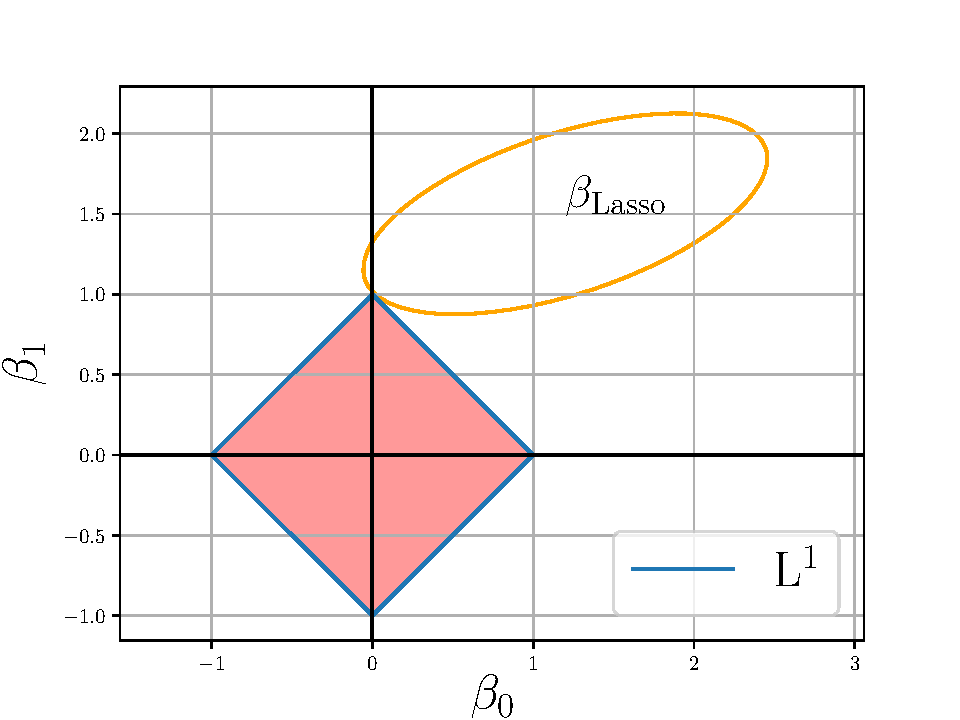
\includegraphics[scale=0.5]{../fig/l1_norm.pdf}
        \caption{L$^1$ norm for Lasso.}
        \label{fig:l1_norm}
    \end{subfigure}%
    \begin{subfigure}[b]{0.5\textwidth}
        \centering
        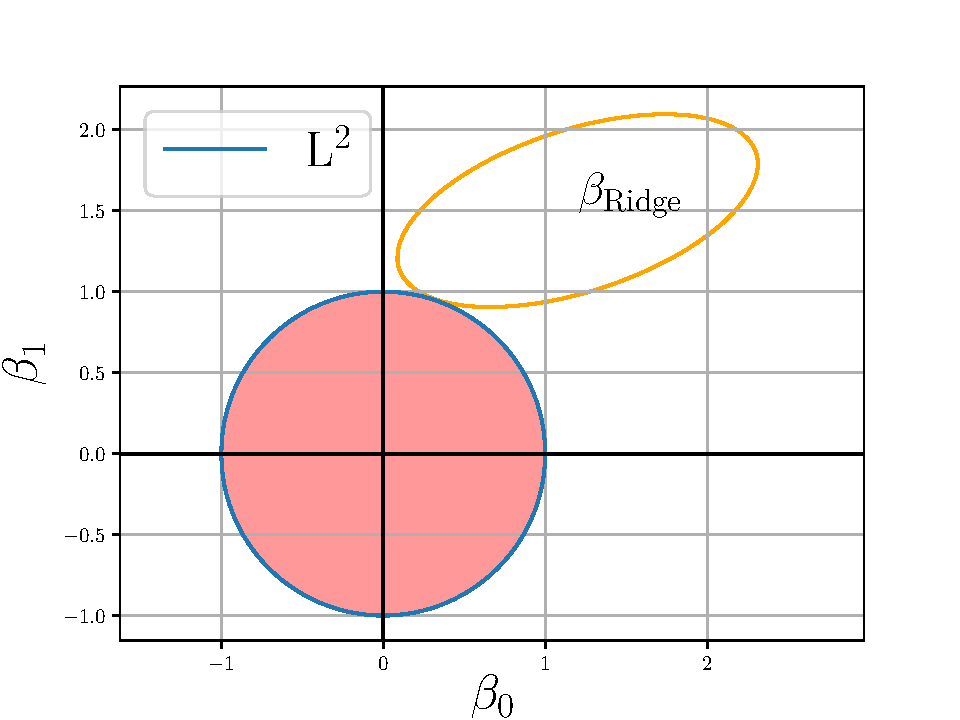
\includegraphics[scale=0.5]{../fig/l2_norm.pdf}
        \caption{L$^2$ norm for Ridge.}
        \label{fig:l2_norm}
    \end{subfigure}
    \caption{In the figure \ref{fig:l2_norm} we see how the search space for the Ridge regression, where we define a success when the $\beta$ parameter hits the circle. The search space for Lasso is viewed on the figure to the right \ref{fig:l1_norm}.}
    \label{fig:norms}
\end{figure}


\subsection{The Bias-Variance decomposition}
It is possible to define variance of the predicted values $\tilde{y}$. If we take the estimator of the general cost function for linear regression \eqref{eq:reg_cost_func},
\begin{align*}
    E[Q(g(\bm{x}))] = E\left[\sum_i (y_i - g(\bm{x_i}))^2 \right]
\end{align*}
it can be shown that we can decompose this into the the variance of $\bm{y}$, bias and noise\cite{2018arXiv180308823M,morten-regression}.
\begin{align}
    \text{MSE} = \text{Bias}^2 + \text{Var} + \text{Noise}
    \label{eq:bias-variance}
\end{align}
The bias is defined as
\begin{align}
    \mathrm{Bias}^2 = \sum_i (\tilde{y}_i - E[\bm{y}])^2,
    \label{eq:bias}
\end{align}
which is measure of how much the prediction deviates from the real data.

A note on the Noise is needed here before we move on. The noise is defined as the the variance in the real data, $\text{Noise}=\text{Var}(\epsilon_\mathrm{noise})$. Since we cannot know the noise beforehand, this will be gobbled up into the bias, as that is a measure of the deviation in real data and prediction. Since the noise is irreducible in the sense we cannot remove the initial noise in the data, the MSE will never lie below $\text{Var}(\epsilon)$ \citep[ch. 2, p. 34]{james2013introduction}.

The variance in \eqref{eq:bias-variance} is defined as the variance in in the prediction, $\tilde{\bm{y}}$.

The MSE in \eqref{eq:bias-variance} is the Mean Square Error is defined as,
\begin{align}
    \text{MSE} = \frac{1}{n} \sum^{n-1}_{i=0}(y_i - \tilde{y}_i)^2,
    \label{eq:mse}
\end{align}
and is simply the averaged squared errors.

% \subsection{Mean Square Error(MSE)}
% The mean square error, popularly called MSE is a function that 
\subsection{\texorpdfstring{$R^2$}{R1} score}
A assessment of the fit quality is given by the $R^2$ score,
\begin{align}
    R^2(\bm{y},\tilde{\bm{y}}) = 1 - \frac{\sum_{i=0}^{n-1}(y_i - \tilde{y}_i)^2}{\sum_{i=0}^{n-1}(y_i - \bar{\bm{y}})^2}
    \label{eq:r2_score}
\end{align}
with $\bar{\bm{y}}$ defined as 
\begin{align*}
    \bar{\bm{y}} = \frac{1}{n}\sum^{n-1}_{i=0} y_i
\end{align*}


\subsection{Determining the best fitting procedure}
An ad-hoc method of determining the best fitting procedure will be used by looking at,
\begin{align}
    \mathrm{Score} = \sqrt{(1-R^2)^2 + (\mathrm{MSE})^2}
    \label{eq:opt_fit}
\end{align}

\subsection{Bootstrapping}
Bootstrapping is a resampling technique particularly useful for small datasets or observables with difficult-to-asses statistics\cite{efron1994introduction}. The bootstrap technique is inspired by the Jackknife method\cite{efron1981}, but differs since we randomly selects a $n$ new samples with replacement of the original dataset $\{y_i\}$ a total of $N_\mathrm{bs}$ times. We use the $N_\mathrm{bs}$ samples to find the MSE, variance and bias. 

A basic for bootstrap algorithm can be set up as following,
\begin{algorithm}[H]
    \caption{Bootstrap}
    \label{alg:bootstrap}
    \begin{algorithmic}[1]
        \State Split the dataset $\bm{X}_{\mathcal{L}}=\{y_i,\bm{x}_i\}$ into a training set and a test set(or holdout set), $\bm{X}_{\mathcal{L},\mathrm{train}}$ and $\bm{X}_{\mathcal{L},\mathrm{test}}$.
        \For{$N_\mathrm{bs}$ times}
            \State Build a new data set $\bm{X}_{\mathcal{L},\mathrm{bs}}=\{y_{i,\mathrm{bs}},\bm{x}_{i,\mathrm{bs}}\}$ with $n$ randomly drawn with replacement values, from the training set $\bm{X}_{\mathcal{L},\mathrm{train}}$.
            \State Fit the bootstrapped dataset to a given model.
            \State Evaluate the model on on the test set $\bm{X}_{\mathcal{L},\mathrm{test}}$.
            \State Store relevant results.
        \EndFor
        \State Perform final statistics on either the collection of bootstrapped datasets and/or take the averages on the stored results. Depending on the type of variable you are sampling, you might need to use latter one.
    \end{algorithmic}
\end{algorithm}

\subsection{\texorpdfstring{$k$}{k}-fold Cross Validation}
The Cross Validation(CV) is a resampling technique which is similar in thought to the Jackknife method, but differs at a few critical places. Details on the $k$-fold CV method can be found in the book An Introduction to Statistical learning by \citet[ch. 5.1]{james2013introduction}, and can be summarized as following,
\begin{algorithm}[H]
    \caption{$k$-fold Cross Validation}
    \label{alg:kfcv}
    \begin{algorithmic}[1]
        \State Shuffle the dataset $\bm{X}_\mathcal{L}=\{y_i,\bm{x}_i\}$.
        \State Split the data set into training and test data, $\bm{X}_{\mathcal{L},\mathrm{train}}$ and $\bm{X}_{\mathcal{L},\mathrm{test}}$.
        \State Split the training data into $k$ \textit{folds}. $\bm{X}_{\mathcal{L},\mathrm{train}}\rightarrow \{\bm{X}_{\mathcal{L},i_k}\}$
        \For{each $i_k$ in the $k$ folds}
            \State Select the sets $\tilde{\bm{X}}_{\mathcal{L}} = \bm{X}_{\mathcal{L}} / \{\bm{X}_{\mathcal{L},i_k}\}$ as training sets, excluding the $k$'th set which is used a holdout set. Note: in order to evaluate the Bias-Variance score \eqref{eq:bias-variance}, the model will not be compared on the $i_k$ test set.
            \State Fit the $\tilde{\bm{X}}_{\mathcal{L}}$ to the model which is being used.
            \State Evaluate the $\tilde{\bm{X}}_{\mathcal{L}}$ on the test set $\bm{X}_{\mathcal{L},\mathrm{test}}$, and perform necessary statistics.
        \EndFor
        \State Summarize the evaluations and statistics gained from the $k$ folds.
    \end{algorithmic}
\end{algorithm}

The Cross Validation comes in many different flavors. Among popular ones are the Monte-Carlo Cross Validation(MCCV). The idea is the same, except that we randomly select the $i_k$'th set to leave out and run this $N_{MC}$ times instead of just $k$ times. The samples selected each time are selected without replacement, but one can have the same samples over many Monte Carlo iterations. E.g. the indices of the first set can be $12, 32, 56, \bm{42}, 94, 83$, and $49, 2, 59, \bm{42}, 51, 73$, where $\bm{42}$ repeats.

\section{Implementation}
The full implementation can be found at \cite{github-repo}. The OLS and Ridge regressions have been implemented, as well as the resampling methods Bootstrap, $k$-fold CV and MCCV. When taking the inverse in OLS regression \eqref{eq:ols_beta_solution} and the inverse in Ridge regression \eqref{eq:ridge-inverse-replacement} in order to find the $\beta$ coefficients a Singular Value Decomposition were used. 

Using scikit-learn\cite{scikit-learn} methods for OLS, Ridge and Lasso regression were implemented, as well as $k$-fold cross validation.

\section{Results}
The results presented are split in two section: the results governing method verification using the Franke function\eqref{eq:franke_function} and methods modeling terrain data as retrieved from \texttt{https://earthexplorer.usgs.gov/}.

\subsection{Verification through the Franke function}
The Franke function $F(x,y)$\eqref{eq:franke_function} maps coordinates $x$, $y$ to a $z$-coordinate. Such a mapping for points $x=[0,1]$, $y=[0,1]$ can be viewed in figure \ref{fig:franke_function}.
\begin{figure}
    \centering
    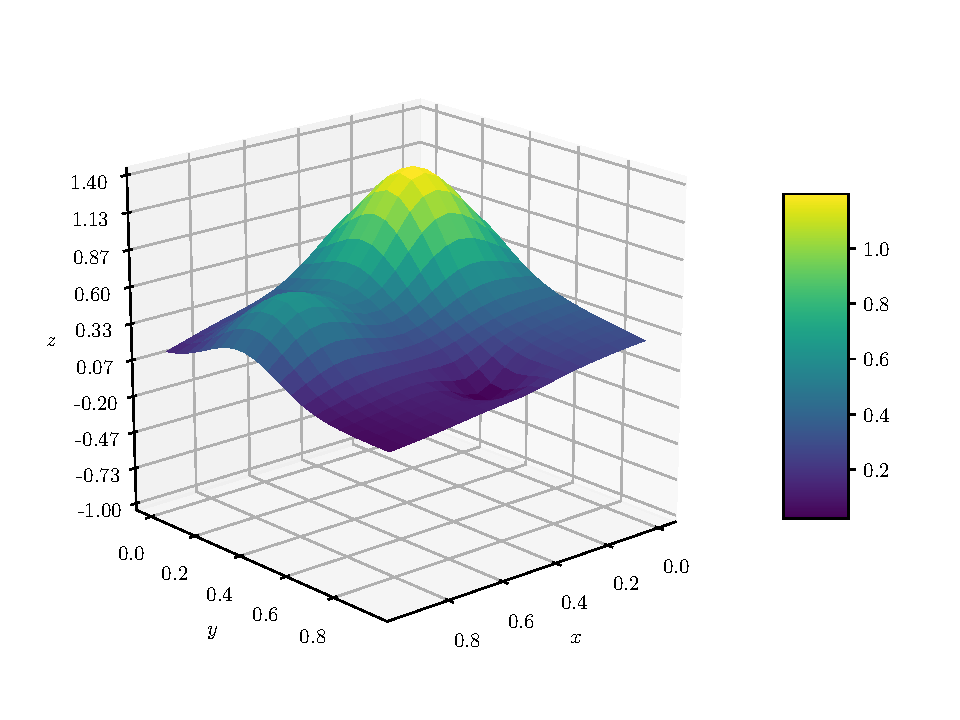
\includegraphics[scale=1.0]{../fig/franke_function.pdf}
    \caption{The mapping of $x=[0,1]$, $y=[0,1]$ through the Franke function \eqref{eq:franke_function}.}
    \label{fig:franke_function}
\end{figure}

In the figure we can see how the 
\begin{figure}
    \centering
    \begin{subfigure}[b]{0.5\textwidth}
        \centering
        \includegraphics[scale=0.5]{../fig/terrain_heatmap.pdf}
        \caption{A plot of $R^2$ versus noise and $\lambda$}
        \label{fig:r2_terrain_heatmap}
    \end{subfigure}%
    \begin{subfigure}[b]{0.5\textwidth}
        \centering
        \includegraphics[scale=0.5]{../fig/terrain_heatmap.pdf}
        \caption{A plot of MSE versus noise and $\lambda$}
        \label{fig:mse_terrain_heatmap}
    \end{subfigure}
    \caption{A plot of how MSE and $R^2$ varies as function of noise and $\lambda$.}
    \label{fig:mse_r2_heatmaps_terrain}
\end{figure}

% \begin{table}[H]
%     \centering
%     \begin{tabular}{l l l l l l} % 6 columns
%         \specialrule{.1em}{.05em}{.05em}
%         Score     & Degree    &$R^2$      & MSE                   & $\mathrm{Bias}^2$     & Var \\ \hline
%         $0.022$      & 5         & $0.98$    & $1.76\cdot 10^{-3}$   & $1.75\cdot 10^{-3}$   & $1.61\cdot 10^{-6}$\\
%         \specialrule{.1em}{.05em}{.05em}
%     \end{tabular}
%     \caption{Based on the different fitting procedures, these fit parameters were determined to be the best. The polynomial fitted was of degree $8$.}
%     \label{tab:opt_result}
% \end{table}
% Optimal score for 
% 'score': 0.021736874931834748, 'r2': 0.9783342056295437, 'mse': 0.0017564413167902263, 'bias': 0.0017489537578899248, 'var': 7.4875589003012656e-06, 'reg_type': 'ols', 'degree': 5,

\begin{figure}[H]
    \centering
    \includegraphics[scale=0.8]{../fig/franke_function_best_fit.png}
    \caption{The optimal fit of the Franke function\eqref{eq:franke_function}, using OLS and polynomial of degree 5.}
    \label{fig:optimal_fit_franke_func}
\end{figure}


\subsection{Modeling terrain}
The terrain we have looked is from a region close to Stavanger in Norway, and can be viewed in figure \ref{fig:terrain_map_full} together with a subset of this region that can be viewed in the sub-figure, \ref{fig:terrain_patch}. We chose a grid of size $100 \times 250$.

\begin{figure}
    \centering
    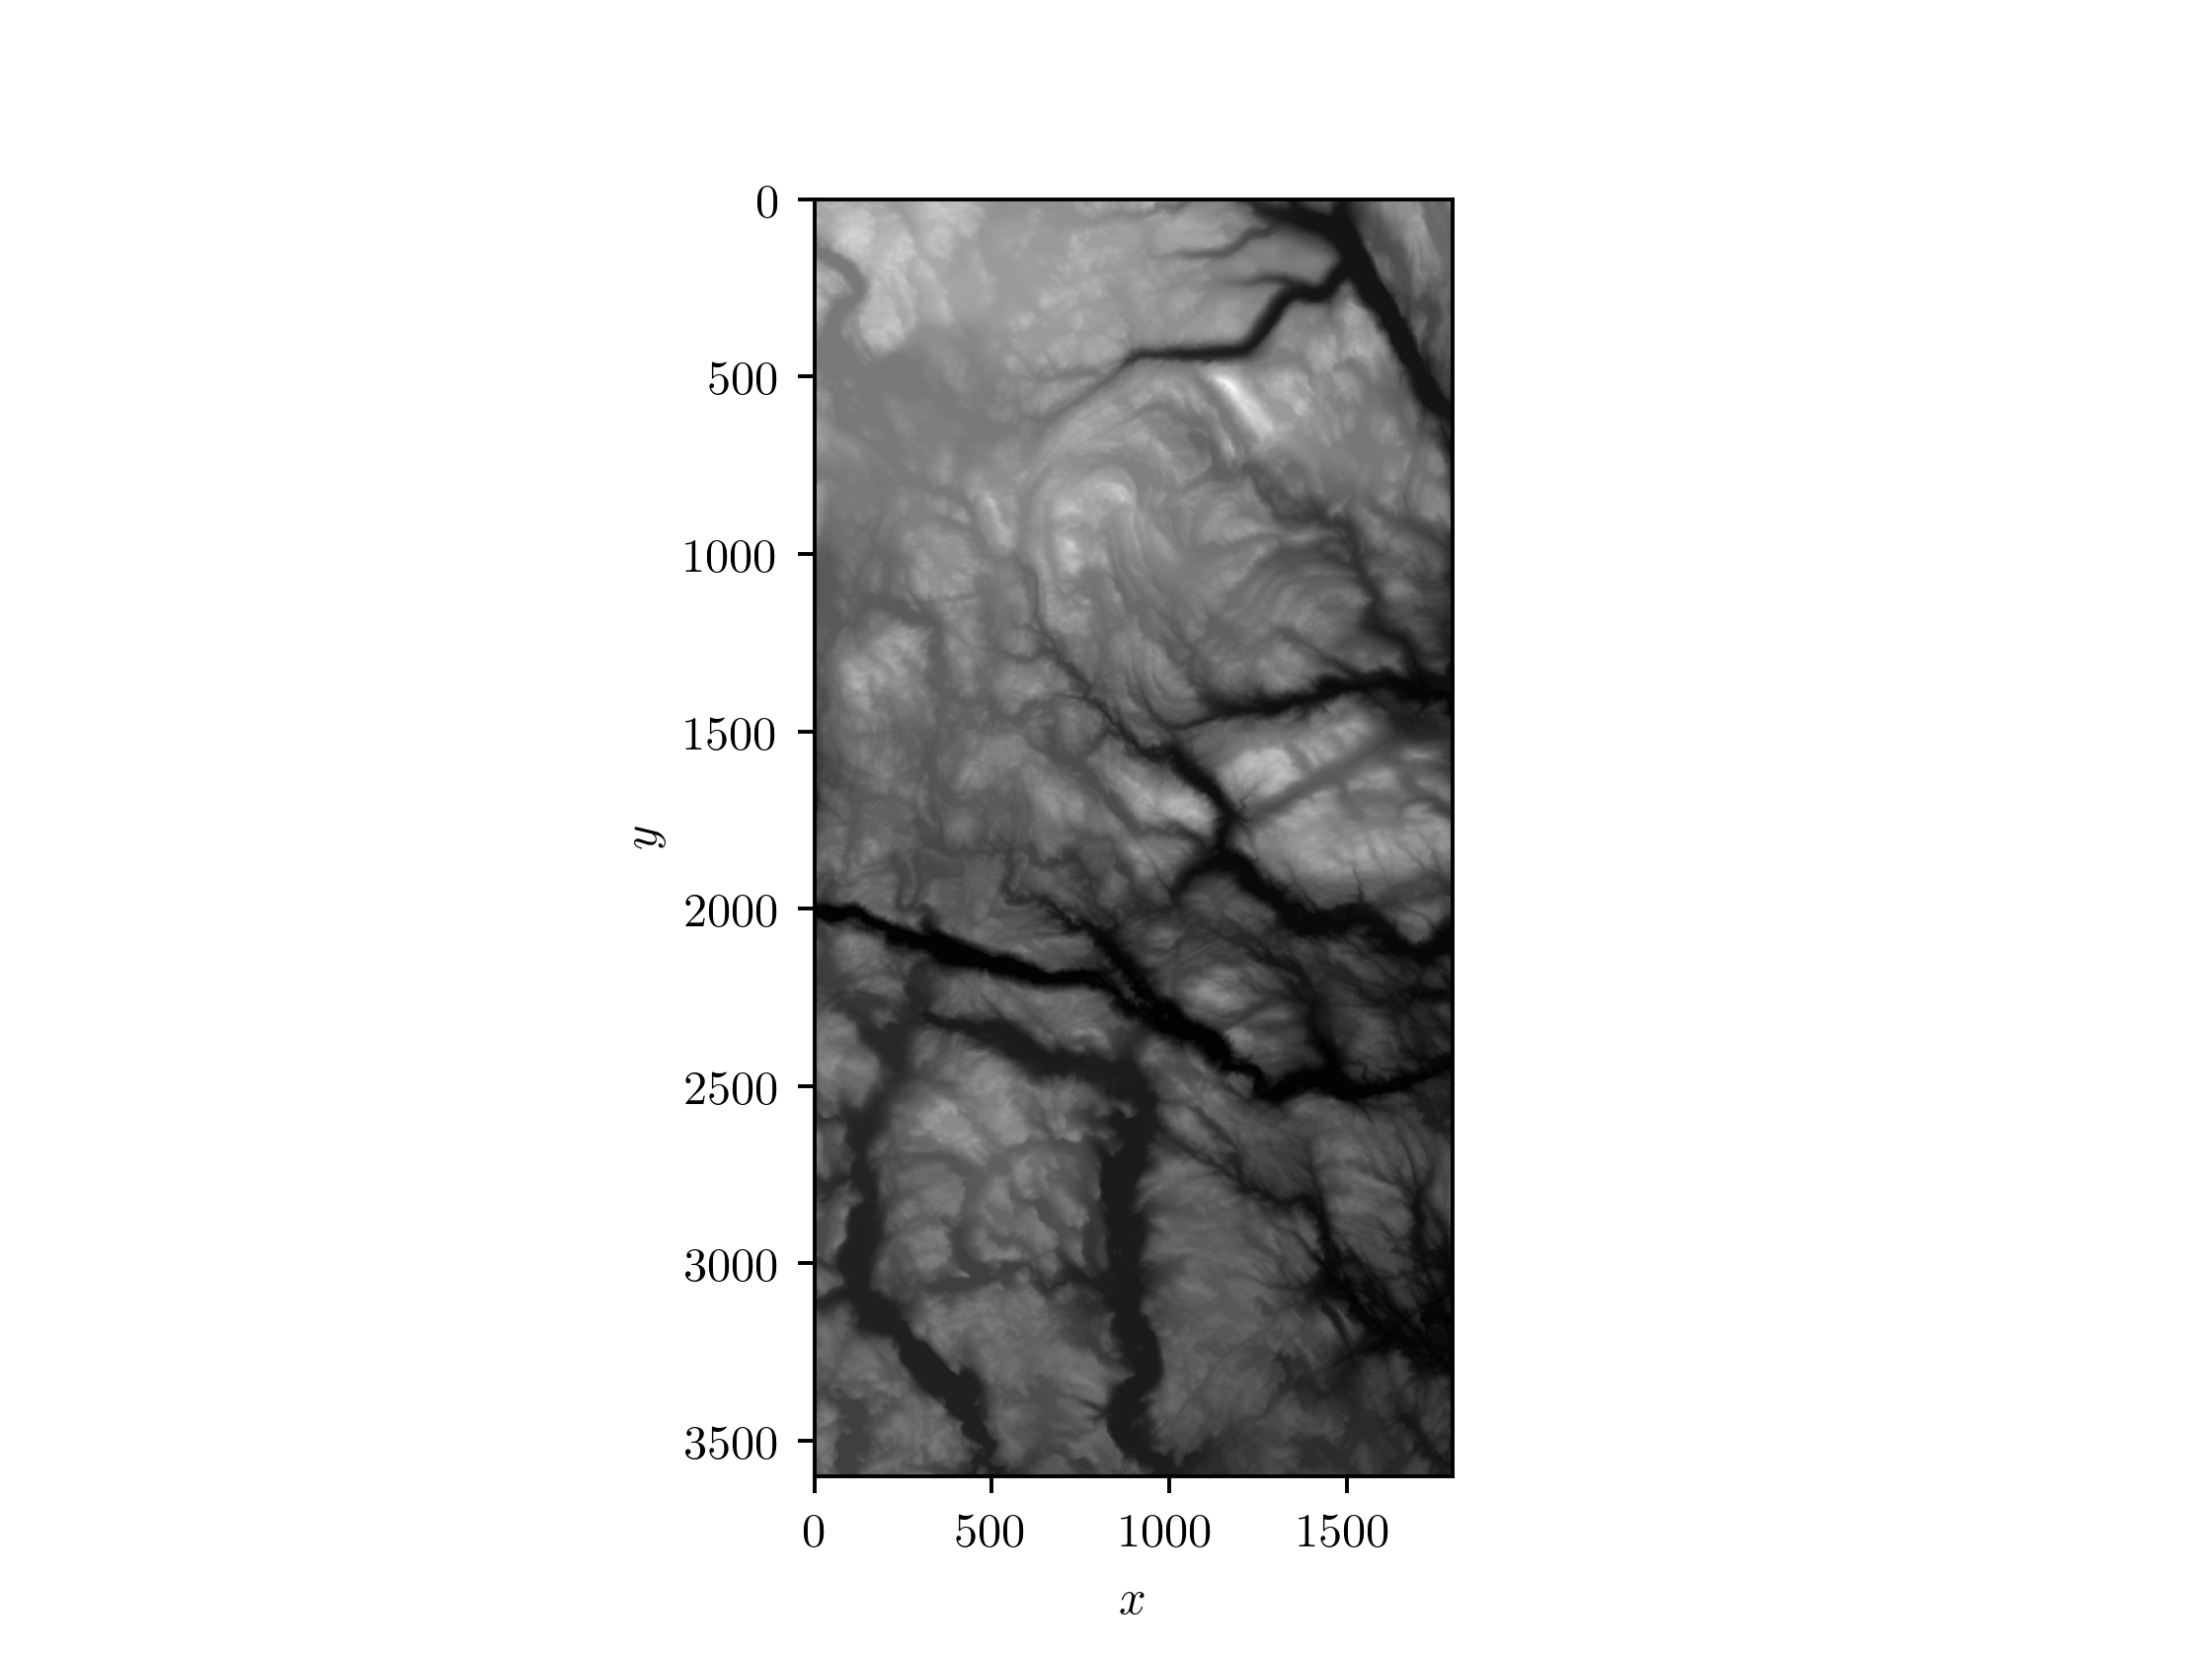
\includegraphics[scale=1.0]{../fig/terrain_data.png}
    \caption{Terrain data from a region close to Stavanger, Norway.}
    \label{fig:terrain_map_full}
\end{figure}

\begin{figure}
    \centering
    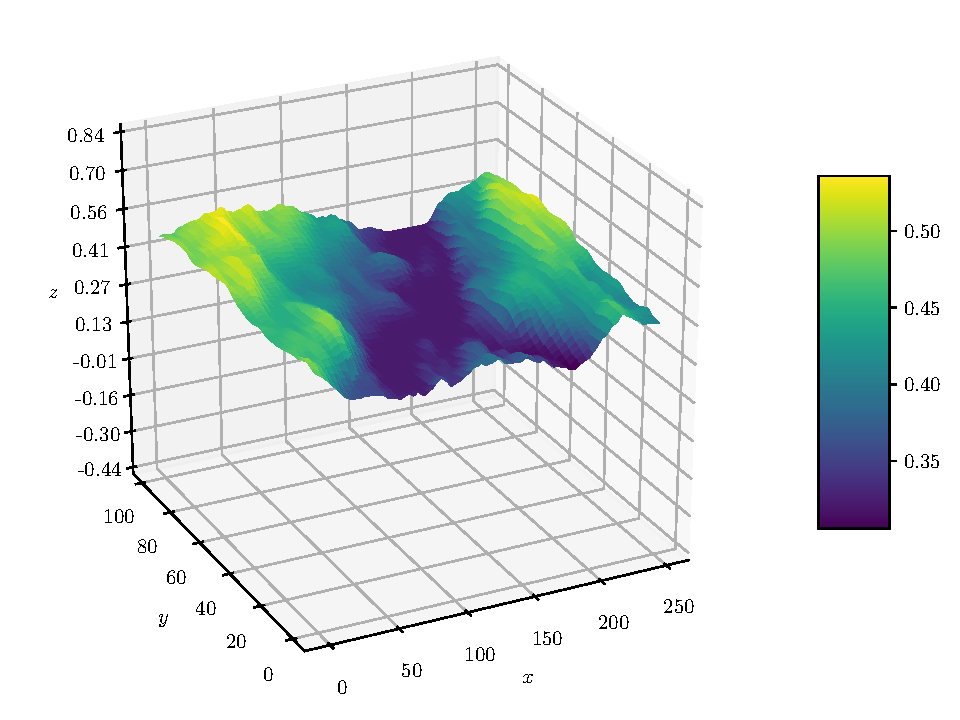
\includegraphics[scale=0.8]{../fig/terrain_patch.pdf}
    \caption{A subset of the region found in figure \ref{fig:terrain_map_full}.}
    \label{fig:terrain_patch}
\end{figure}

The optimal fit method was found by looking at the $R^2$ and MSE values\eqref{eq:opt_fit}. The result was that the Lasso method proved to be the most effective, as summed up in table \ref{tab:opt_result}. The figure which these parameters replicates in terms of terrain features can be viewed in figure \ref{fig:optimal_fit}.
\begin{table}[H]
    \centering
    \begin{tabular}{l l l l l l l} % 6 columns
        \specialrule{.1em}{.05em}{.05em}
        Score     & Degree    &$R^2$      & MSE                   & $\mathrm{Bias}^2$     & Var                   & $\lambda$ \\ \hline
        $0.12$      & $8$         & $0.88$    & $1.72\cdot 10^{-3}$   & $1.72\cdot 10^{-3}$   & $1.61\cdot 10^{-6}$   & $10^{-4}$ \\
        \specialrule{.1em}{.05em}{.05em}
    \end{tabular}
    \caption{Based on the different fitting procedures, these fit parameters were determined to be the best. The polynomial fitted was of degree $8$.}
    \label{tab:opt_result}
\end{table}

\begin{figure}[H]
    \centering
    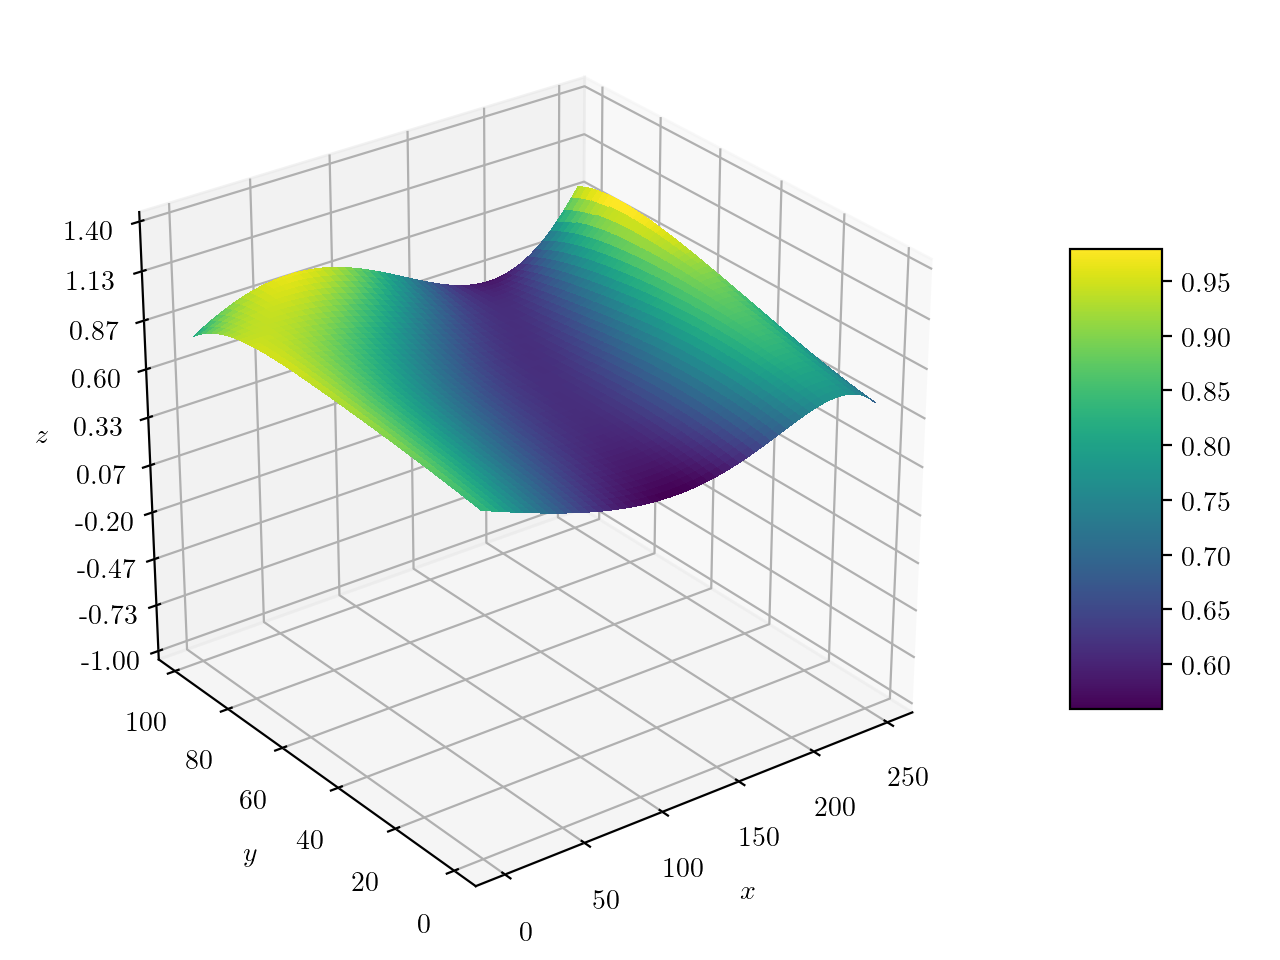
\includegraphics[scale=0.8]{../fig/lasso_fit_deg8.png}
    \caption{The optimal fit of the terrain data. Determined to be by a polynomial of degree 8 with the Lasso method.}
    \label{fig:optimal_fit}
\end{figure}


\section{Discussion and conclusion}


\begin{appendices}
\subsection{The Franke Function} \label{sec:appendix}
The Franke function as given in \cite{franke1979critical},
\begin{align}
    F(x,y) &= 0.75\exp\left(-\left(0.25\left(9x-2\right)^2\right) - 0.25\left(\left(9y-2\right)^2\right)\right) \\
    &= 0.75\exp\left(-\frac{1}{49}\left(\left(9x+1\right)^2\right) - 0.1\left(9y+1\right)\right) \\
    &= 0.5\exp\left(-\left(9x-7\right)^2/4.0 - 0.25\left(\left(9y-3\right)^2\right)\right) \\
    &= -0.2\exp\left(-\left(9x-4\right)^2 - \left(9y-7\right)^2\right)
    \label{eq:franke_function}
\end{align}
\end{appendices}

\bibliography{bib/bibliography.bib}
\bibliographystyle{plainnat}


\end{document}